#import "@local/bootlin:0.1.0": *

#import "@local/bootlin-yocto:0.1.0": *

#import "@local/bootlin-utils:0.1.0": *

#import "../../typst/local/themeBootlin.typ": *

#import "../../typst/local/common.typ": *

#show: bootlin-theme.with( aspect-ratio: "16-9", config-common(handout: "handout" in sys.inputs and sys.inputs.handout == "1", ))

#show raw.where(block: true): set block(fill: luma(240), inset: 1em, radius: 0.5em, width: 100\%)

#show raw.where(block: true): set text(size: 11pt)

#show raw.where(block: false): r => text(fill: color-link)[#r]

#show raw.where(lang: "c", block: true): set block(fill: luma(240), inset: 0.4em, radius: 0.5em, width: 95\%, breakable: true, above: 12pt, below: 12pt)

#show raw.where(lang: "c", block: true): set text(11pt)

#show raw.where(lang: "console", block: true):set block(fill: luma(240), inset: 0.4em, radius: 0.5em, width: 95\%, breakable: true, above: 6pt)

#show raw.where(lang:"console", block: true): set text(12pt)

 = Hardware initialization

=== Hardware initialization

#columns(gutter: 8pt)[
The hardware needs time to initialize
\begin{itemize}
\item Voltage regulation, crystal stabilization
\item Can be up to 200 ms
\item As a software developer, you can't do anything about this part.
\item All you can do is measure this time with an oscilloscope and
      ask the hardware board designers whether the can do anything about
      this. However, there are delays in the CPU which may not be
      possible to reduce (see the CPU datasheet).
\end{itemize}
 #colbreak()
% From % https://openclipart.org/detail/28106/processor_clock-by-klaasvangend
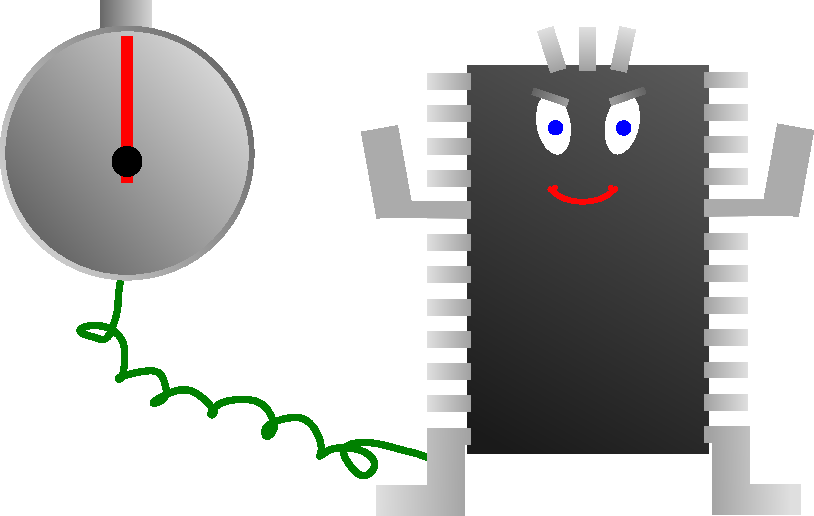
\includegraphics[width=\textwidth]{slides/boot-time-hardware-init/klaasvangend_processor_clock.pdf}
\\]


